\input{../../main}

\begin{document}

\setphysstyle{ГЦФО 8}{Серия Ш-01}{14.09.2016}

\Large

\task{ Человек бежит по эскалатору. В первый раз он насчитал 50
  ступенек. Во второй раз, двигаясь в ту же сторону со скоростью в три
  раза большей, он насчитал 75 ступенек. Сколько ступенек насчитал бы
  человек на неподвижном эскалаторе? }
% Русаков, 1.7

\task{ Плот и моторная лодка одновременно начинают движение из пункта
  \textbf{A}. Лодка проходит путь $AB=S_1$ за время $t$ и возвращается
  обратно. На расстоянии $BC=S_2$ лодка встречает плот
  (см. рис.). Найти скорость течения и собственную скорость
  лодки. Решите эту задачу в системе отсчёта а) земли; б) лодки; в)
  плота.
  \begin{center}
    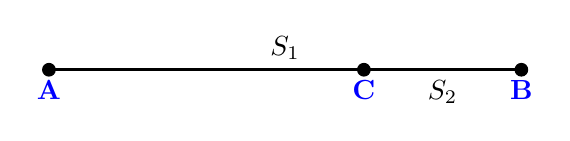
\begin{tikzpicture}
      \draw[very thick] (0,0) node[below,blue] {\textbf{A}} --
      (4,0) node[below,blue] {\textbf{C}} -- (6,0) node[below,blue]
      {\textbf{B}} node[below,midway] {$S_2$};
      \draw (0,0) -- (6,0) node[above,midway] {$S_1$};
      \draw[fill=black] (0,0) circle (0.08cm);
      \draw[fill=black] (4,0) circle (0.08cm);
      \draw[fill=black] (6,0) circle (0.08cm);        
    \end{tikzpicture}
  \end{center}
}
% Шапиро-Бодик-1, стр. 11

\task{ Колонна бегунов имеет скорость $v$ и длину $l$. Навстречу
  бегунам бежит тренер со скоростью $u$ ($u<v$). Поравнявшись с
  тренером, каждый бегун поворачивает в противоположном направлении и
  бежит со скоростью $v$. Какова будет длина колонны, когда тренер
  поравняется с последним бегуном? Решите эту задачу в системе отсчёта
  а) тренера; б) колонны бегунов; в) земли. }
% Шапиро-Бодик-1, стр. 11

\task{ Кольцо сварено из двух полуколец радиуса $R$, скорости звука в
  которых равны $c_1$ и $c_2$. Через какое время встретятся звуковые
  волны, возбуждённые ударом по точке сварки? Длина окружности радиуса
  $R$ равна $2\pi R$. }
% нгу-1, 1.2
            
\end{document}

%%% Local Variables: 
%%% mode: latex
%%% TeX-engine:xetex
%%% TeX-PDF-mode: t
%%% End:
